\documentclass[professionalfonts, xcolor={usenames,svgnames,x11names,table}]{beamer}

\usetheme{SBUclass}
\usepackage{mypackages}
\usepackage{mycommands}


\title{\texorpdfstring{Exploring Lexical Semantics \\with Word Embeddings}{}}
\author[DeSanto]{\texorpdfstring{%
                            \textbf{Aniello De Santo}                            }
                            {Aniello De Santo} 
                        }
\institute{
\texttt{aniellodesanto.github.io\\aniello.desanto@stonybrook.edu}
    \begin{tikzpicture}[remember picture, overlay]
        \node[draw=Red3, fill=Red3!25, thick, align=center]
            (hint) at ($(current page.center) + (15em,-3em)$)
            {Get the slides!};
              % \draw[Red3,thick,-{Latex[length=.5em]}] (hint) - + (-2em,0em);
            % \draw[Red3,thick,-{Latex[length=.5em]}] (hint) - + (-1.5em,1.5em);
               \draw [Red3,thick,-{Latex[length=.5em]}] (hint) edge ($(current page.center) + (15em,-5em)$) ;
    %     \draw[Red3,thick,-{Latex[length=.5em]}] (hint) |- +(-4.5em,4.25em);
            \node[inner sep=0pt]  (hint2) at ($(current page.center) + (15em,-10em)$) {
\includegraphics[width=0.25\linewidth]{img/QR_slides.png}};
    \end{tikzpicture}

}
\date{San Jose State\\ Feb 6, 2020}
%%%%%%%%



\begin{document}
\unnumbered{
\begin{frame}
	\titlepage
\end{frame}
}
%

\begin{frame}{Word Meanings}
    \begin{itemize}
        \item What is a word meaning?
    \end{itemize}

\visible<2->{
    \begin{exampleblock}{Example: Dictionary Approach}
        \textbf{dog}
        \begin{itemize}
            \item is a \textbf{mammal},
            \item descended from \textbf{wolf},
            \item is commonly a \textbf{pet},
            \item subtypes are \textbf{poodle}, \textbf{bulldog}, \ldots
            \item has \textbf{fur},
            \item \ldots
        \end{itemize}
    \end{exampleblock}
    }
    % fixme: use wordnet here
\end{frame}

\begin{frame}{Wordnet}
\begin{center}
        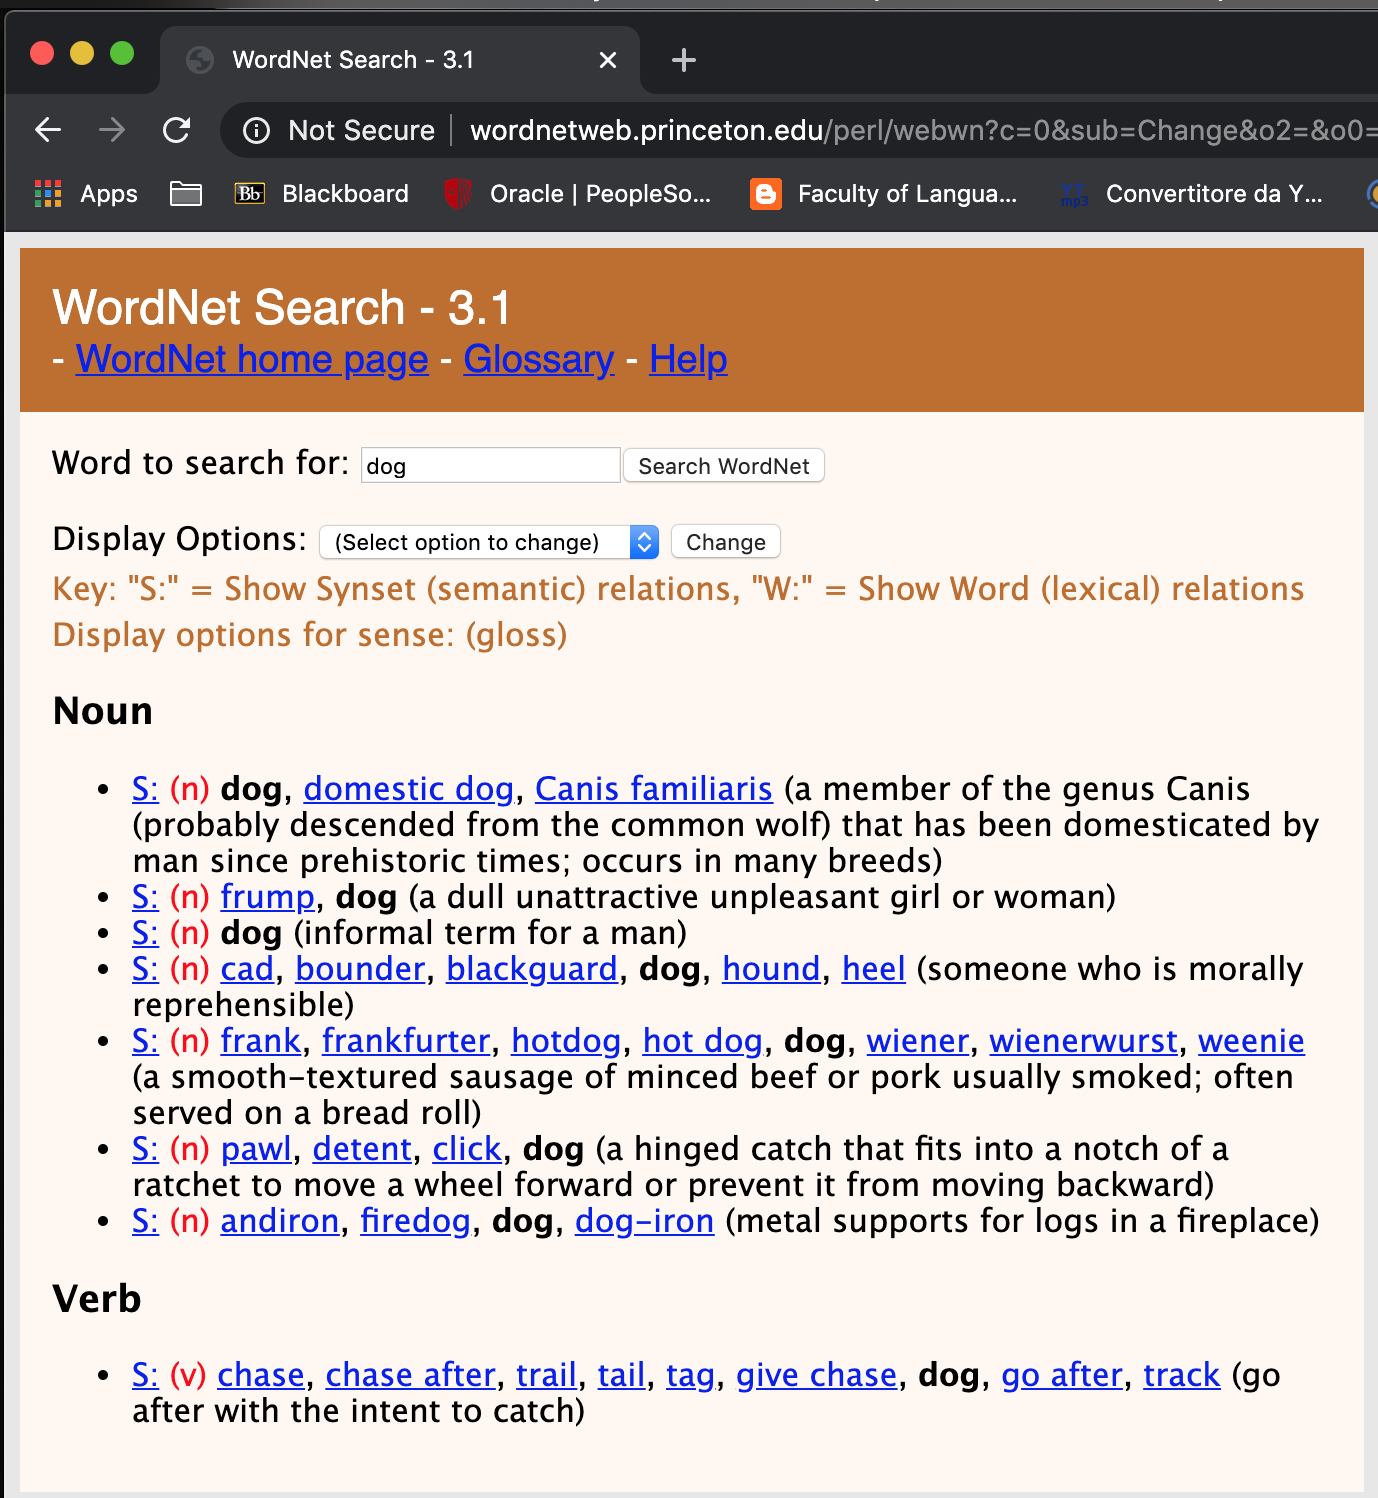
\includegraphics[width=0.7\linewidth]{./img/wordnet3}

\end{center}
\end{frame}


\begin{frame}{Why the Dictionary Approach is Problematic}
    \begin{itemize}
        \item Such dictionaries have been tried for computers.\\
            \subpoint{e.g. \href{https://wordnet.princeton.edu/}{WordNet}}
        \item They must be created by hand, which is a big problem:
            \begin{itemize}
                \item expensive
                \item only available for some languages
                \item many new words missing
            \end{itemize}
        \item We need dictionaries that can be generated automatically.
    \end{itemize}
\end{frame}

\begin{frame}{Meaning as Word Use}
    \begin{columns}
        \column{.7\linewidth}
        \begin{itemize}
            \item The philosopher \textbf{Ludwig Wittgenstein} said that a word's meaning is its use.
        \end{itemize}
        \begin{block}{Computational Counterpart}
            A word's meaning is given by how often it occurs together with other words.
        \end{block}
        
        \column{.3\linewidth}
        \centering
        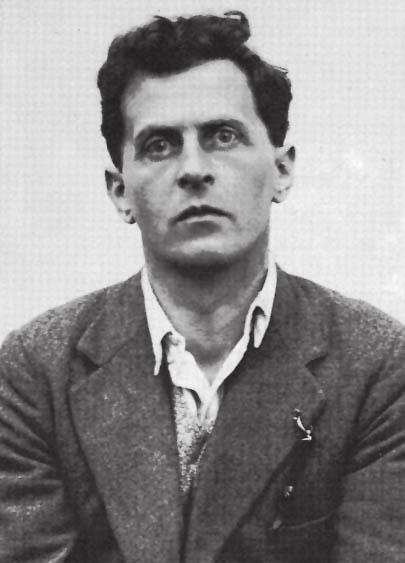
\includegraphics[width=1\linewidth]{./img/wittgenstein}
    \end{columns}
\end{frame}

\begin{frame}{Counting Tokens for Word Meaning}
    \textbf{Step 1:} Record in how many sentences words \highlight{occur together}
    %
    \begin{example}
        \begin{quote}
            The dog barked at the cat.
            The cat ran away.
            The dog ran after the cat.
            The dog kept barking.
            He also kept running.
        \end{quote}
        %
        \centering
            \begin{tabular}{r|cccc}
                           & dog & cat & bark & run\\
                    \hline
                    dog    & -   & \visible<2->{2}   & \visible<3->{2}    & \visible<4->{1}\\
                    cat    & \visible<5->{2}   & -   & \visible<6->{1}    & \visible<7->{2}\\
                    bark   & \visible<8->{2}   & \visible<9->{1}   & -    & \visible<10->{0}\\ 
                    run    & \visible<11->{1}   & \visible<12->{2}   & \visible<13->{0}    & -\\
            \end{tabular}
    \end{example}
\end{frame}

\begin{frame}{From Vectors to Vector Spaces}
    \textbf{Step 2:} Construct an $n$-dimensional vector space.\\
    \subpoint{\qquad\qquad $n$ is given by the number of word types in the text}
    %
    \begin{exampleblock}{2-Dimensional Vector Space with \emph{dog} and \emph{cat}}
        %
        \begin{columns}
            \column{.3\linewidth}
            \centering
                \begin{tikzpicture}
                    \node (top) at (0em,10em) {};
                    \node (start) at (0,0) {};
                    \node (right) at (10em,0em) {};

                    \foreach \x in {4em,8em}
                        {
                        \draw[gray] (\x, .25em) -- (\x, -.25em);
                        \draw[gray] (.25em, \x) -- (-.25em, \x);
                        }

                    \draw[->,gray] (start.center) to node [above,pos=1] {dog} (top);
                    \draw[->,gray] (start.center) to node [right,pos=1] {cat} (right);

                    \draw[->,SteelBlue4] (start.center) to node [left, pos=.9] {bark} (4em,8em);
                    \draw[->,Red3] (start.center) to node [below, pos=.9] {run} (8em,4em);
                \end{tikzpicture}

            \column{.55\linewidth}
            \begin{center}
                \begin{tabular}{r|cccc}
                               & dog & cat & bark & run\\
                        \hline
                        dog    & -   & {2}   & {2}    & {1}\\
                        cat    & {2}   & -   & {1}    & {2}\\
                        bark   & \tikz[overlay,remember picture, baseline=-.7ex]{\node (bd) {2};}
                               & \tikz[overlay,remember picture, baseline=-.7ex]{\node (bc) {1};}
                               & -    & {0}\\ 
                        run    & \tikz[overlay,remember picture, baseline=-.7ex]{\node (rd) {1};}
                               & \tikz[overlay,remember picture, baseline=-.7ex]{\node (rc) {2};}
                               & {0}    & -\\
                \end{tabular}
                \begin{tikzpicture}[overlay, remember picture]
                    \draw[draw=Purple, fill=Purple, thick, fill opacity=.25]
                        (bd.north west) rectangle (rc.south east);
                \end{tikzpicture}
            \end{center}
            \begin{itemize}
                \item \emph{bark} more closely related to \emph{dog}
                \item \emph{run} more closely related to \emph{cat}
            \end{itemize}
        \end{columns}
    \end{exampleblock}
\end{frame}

%\begin{frame}{From Word Meaning to Text Meaning}
%    \textbf{Step 3}: construct vector for whole text from word vectors
%
%    \begin{exampleblock}{Meaning for \emph{He either barks or runs and barks}}
%        \centering
%        \begin{tikzpicture}
%            \node (top) at (0em,10em) {};
%            \node (start) at (0,0) {};
%            \node (right) at (10em,0em) {};
%
%            \foreach \x in {4em,8em}
%                {
%                \draw[gray] (\x, .25em) -- (\x, -.25em);
%                \draw[gray] (.25em, \x) -- (-.25em, \x);
%                }
%
%            \draw[->,gray] (start.center) to node [above,pos=1] {dog} (top);
%            \draw[->,gray] (start.center) to node [right,pos=1] {cat} (right);
%
%            \draw[->,SteelBlue4] (start.center) to node [left, pos=.9] {bark} (4em,8em);
%            \draw[->,Red3] (start.center) to node [below, pos=.9] {run} (8em,4em);
%            \draw[->,Purple] (start.center) to node [right, pos=.9] {text} (5em,7em);
%        \end{tikzpicture}
%    \end{exampleblock}
%\end{frame}

\begin{frame}{Problems?}
   \begin{itemize}
        \item \textbf{Conceptual Concerns}
            \begin{itemize}
               	 \item Is word meaning really just a bunch of numbers?
               \end{itemize}
       \end{itemize} 
      
      \vspace{0.3cm} 
      \begin{itemize}           
        \item \textbf{(More) Practical Concerns}
               \begin{itemize}
                \item In a real-word model, the vector space will have\\
                    thousands of dimensions (thousands of unique words)
                    \item most of the words in the vocabulary will not co-occur in the same sentence (or document!)\\
                    $\Rightarrow$ results in vectors with mostly empty (zeros) slots.
                      \item Will similar words have similar vectors?
                         \end{itemize}
                            \end{itemize}

\end{frame}


\begin{frame}{Word Embedding Methods}
\centering 

\begin{table}[]
\begin{tabular}{ll}
\hline
\multicolumn{1}{c}{Method} & \multicolumn{1}{c}{Paper}   \\ \hline  \hline
LSA                        & Landauer \& Dumais (1997)   \\
Word2Vec                   & Mikolov et al.  (2013)      \\
ELMo                       & Peters et al.  (2018)       \\
BERT                       & Devlin et al. (2019, arxiv) \\ \hline
\end{tabular}
\end{table}

\pause
\begin{alertblock}{Word2Vec}
\begin{itemize}
	\item Word2Vec is  \textbf{predictive model} for learning word embeddings from raw text
	\item  a shallow, two-layer neural networks trained to reconstruct linguistic contexts of words
	\item words that share common contexts in the corpus are located in close proximity to one another in the space
\end{itemize}
\end{alertblock}

\end{frame}

%\begin{frame}{Word2Vec}
%
%\begin{itemize}
%\item Word2Vec is  \textbf{predictive model} for learning word embeddings from raw text
%\item  a shallow, two-layer neural networks trained to reconstruct linguistic contexts of words
%\item words that share common contexts in the corpus are located in close proximity to one another in the space
%\end{itemize}
%
%
%\end{frame}


\begin{frame}{A Quick Excursus: The Perceptron}
    \begin{block}{The Perceptron: A Mini-Version of a Neural Network}
        \begin{itemize}
            \item \textbf{input layer:} neurons that are sensitive to input
            \item \textbf{output layer:} neurons that represent output values
            \item \textbf{connections:} weighted links between input and output layer
            \item most activated output neuron represents decision
        \end{itemize}
    \end{block}
    %
    \begin{center}
        \begin{tikzpicture}
            \node[minimum size=3em,draw,circle] (dear) at (0,0) {Dear};
            \node[minimum size=3em,draw,circle] (hi) [left=of dear] {Hi};
            \node[minimum size=3em,draw,circle] (emily) [right=of dear] {Emily};
            \node[minimum size=3em,draw,circle] (ham) [below=5em of hi] {ham};
            \node[minimum size=3em,draw,circle] (spam) [below=5em of emily] {spam};

            \foreach \Input/\Output/\Value in {%
                    dear/ham/0,
                    dear/spam/5,
                    hi/ham/3,
                    hi/spam/1,
                    emily/ham/10,
                    emily/spam/0}
                \draw[->] (\Input) to node [right, pos=.75] {\Value} (\Output);
        \end{tikzpicture}
    \end{center}
\end{frame}

\begin{frame}{Perceptron Activation for \emph{Hi Dear}}
    \begin{center}
        \begin{tikzpicture}
            \node[minimum size=3em,draw,circle,fill=blue!25] (dear) at (0,0) {Dear};
            \node[minimum size=3em,draw,circle,fill=blue!25] (hi) [left=of dear] {Hi};
            \node[minimum size=3em,draw,circle] (emily) [right=of dear] {Emily};
            \node[minimum size=3em,draw,circle,fill=red!10] (ham) [below=5em of hi] {ham};
            \node[minimum size=3em,draw,circle,fill=red!35] (spam) [below=5em of emily] {spam};

            \foreach \Input/\Output/\Value in {%
                    dear/ham/0,
                    dear/spam/5,
                    hi/ham/3,
                    hi/spam/1,
                    emily/ham/10,
                    emily/spam/0}
                \draw[->] (\Input) to node [right, pos=.75] {\Value} (\Output);
        \end{tikzpicture}
    \end{center}
\end{frame}

\begin{frame}{Perceptron Activation for \emph{Hi Dear Emily}}
    \begin{center}
        \begin{tikzpicture}
            \node[minimum size=3em,draw,circle,fill=blue!25] (dear) at (0,0) {Dear};
            \node[minimum size=3em,draw,circle,fill=blue!25] (hi) [left=of dear] {Hi};
            \node[minimum size=3em,draw,circle,fill=blue!25] (emily) [right=of dear] {Emily};
            \node[minimum size=3em,draw,circle,fill=red!75] (ham) [below=5em of hi] {ham};
            \node[minimum size=3em,draw,circle,fill=red!35] (spam) [below=5em of emily] {spam};

            \foreach \Input/\Output/\Value in {%
                    dear/ham/0,
                    dear/spam/5,
                    hi/ham/3,
                    hi/spam/1,
                    emily/ham/10,
                    emily/spam/0}
                \draw[->] (\Input) to node [right, pos=.75] {\Value} (\Output);
        \end{tikzpicture}
    \end{center}
\end{frame}


\begin{frame}{Back to Word2Vec}

\begin{itemize}
\item  A NN trained to reconstruct linguistic contexts of words
\item Two learning algorithms:
	\begin{itemize}
	\item the Continuous Bag-of-Words (CBOW) 
	\item \alert<2->{the Skip-Gram model}\visible<3->{:  predict \alert{context} based on \alert{target} word.}
	\end{itemize}
\end{itemize}


\begin{center}
        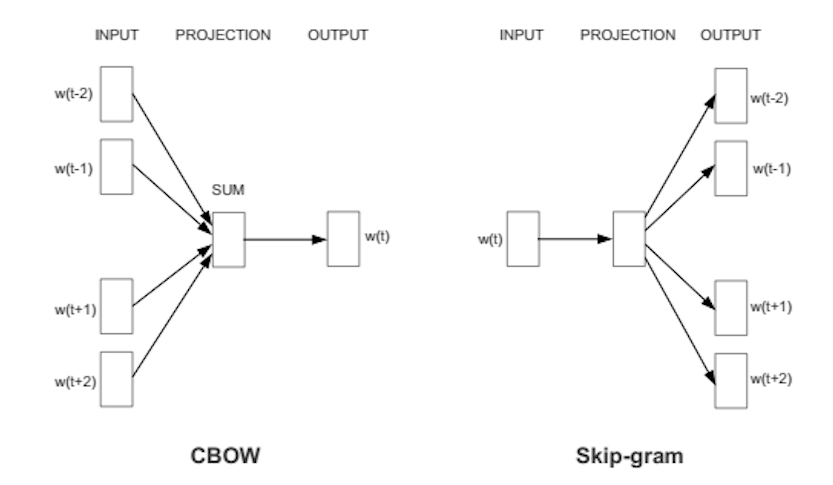
\includegraphics[width=0.8\linewidth]{./img/models_comp}
\end{center}

\end{frame}

\begin{frame}{The Skip-Gram Model: Architecture}

\begin{center}
        \includegraphics[width=0.85\linewidth]{./img/skip_gram3}
\end{center}

\vspace{-0.2cm}
\resizebox{.7\textwidth}{!}{% 
 \begin{table}[]
\begin{tabular}{|l|l|l|l|l|l|l|l|l|l|}
\hline
0.3 & 0.1 & 0.38 & 0.22 & 0.05 & 0.09 & ... & 0.98 & 0.13 & 0.2\\ \hline
\end{tabular}
\end{table}
}
\end{frame}



\begin{frame}{The Skip-Gram Model: Predicting Context}

	\begin{itemize}
	\item Skip-Gram: predict \alert{context} based on \alert{target} word.
	\end{itemize}

\begin{center}
        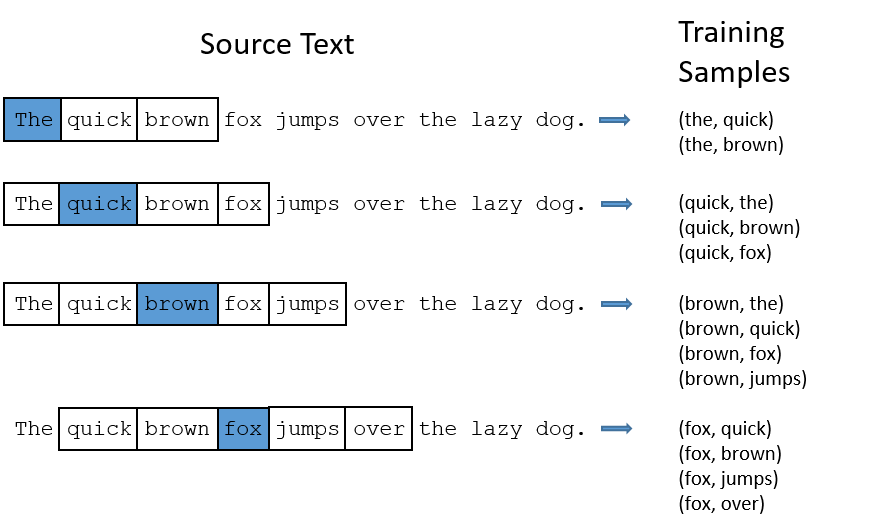
\includegraphics[width=1\linewidth]{./img/skip_gram_training}
\end{center}
\end{frame}


\begin{frame}[plain]
    \begin{center}
        \begin{tikzpicture}
            \node[draw=Red3,fill=Red3!25,thick,
                  font=\LARGE\bfseries, align=center,
                  inner sep=1em] at (0,0) %
                {Let's try it together!};
        \end{tikzpicture}
    \end{center}
    \vspace{1cm}
    \begin{columns}
\begin{column}{0.5\textwidth}
\centering
    
\includegraphics[width=0.5\linewidth]{img/QR_tutorial.png}
    \end{column}
    \begin{column}{0.5\textwidth}
    \centering
    \href{shorturl.at/ADPSX}{\large{\alert{\textbf{shorturl.at/ADPSX}}}}
        \end{column}
            \end{columns}
\end{frame}


\begin{frame}{Some Recent Applications}
    \begin{itemize}
        \item \textbf{Web Search}
            \begin{itemize}
                \item construct meaning vector for every website
                \item rank websites by vector similarity
            \end{itemize}
        \item \textbf{Ad Sense}
            \begin{itemize}
                \item associate every ad with a vector
                \item pick ad that most closely matches website vector
            \end{itemize}
    \end{itemize}

    \begin{block}{Possible Concerns}
 \begin{itemize}
                    \item Watch out for \alert{\textbf{intrinsic biases}!}
            \end{itemize}
    \end{block}
\end{frame}

\begin{frame}{The Danger of Corpora}

\begin{center}
        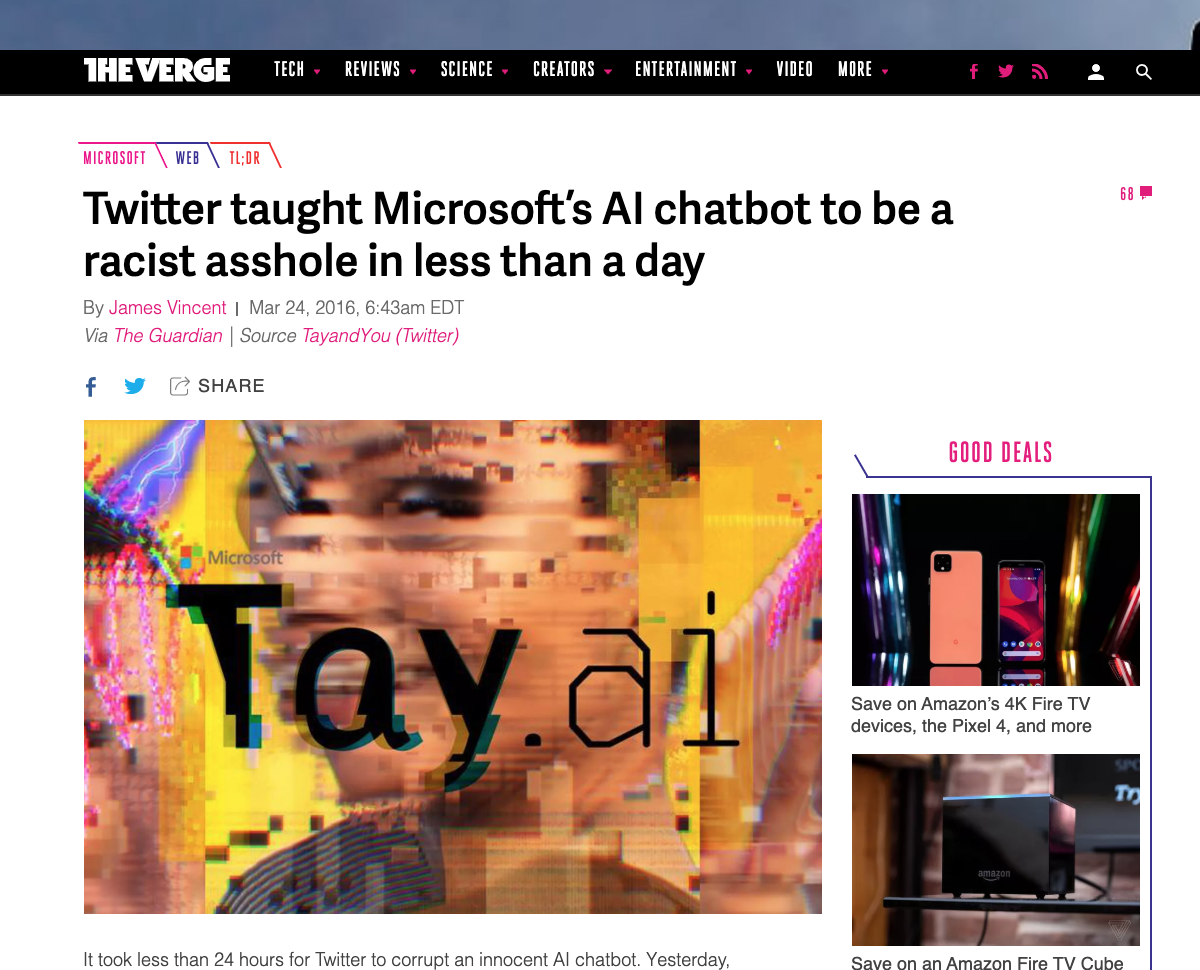
\includegraphics[width=1\linewidth]{./img/bias1}
\end{center}

\end{frame}

\begin{frame}{Is This Realistic?}
    \begin{itemize}
        \item \textbf{Possible Concerns}
            \begin{itemize}
                \item Is word meaning really just a bunch of numbers?
            \end{itemize}
        \item But this might actually capture something psychologically real!
    \end{itemize}
    %
    \begin{block}{Psycholinguistic Experiments}
        \begin{itemize}
            \item Word association tasks (Rubistein et al. 2015)
             \item ERP measures of context appropriateness \\ (Broderik et al. 2018, Ettinger et al. 2016)
              \item  Priming effects (Gunther et al. 2016)
                 \begin{itemize}
               \item Check it out: \href{http://www.u.arizona.edu/~kforster/priming/index.htm}{\textbf{Masked priming effects!}}
       		 \end{itemize}
         \end{itemize}
    \end{block}
\end{frame}

\begin{frame}{Is This Realistic? [cont.]}
    \begin{itemize}
        \item For word meaning, the approach seems to work.
        \item But what about sentence/text meaning?
    \end{itemize}
    %
    \begin{example}
        The following two sentences receive the same vector:
        %
        \begin{exe}
            \ex
            \begin{xlist}
                \ex Dog bites man!
                \ex Man bites dog!
            \end{xlist}
        \end{exe}
    \end{example}
    %
\end{frame}

\begin{frame}{Is This Realistic? [cont.]}

\begin{columns}
\begin{column}{0.5\textwidth}
    \begin{itemize}
        \item Meaning is not just about lexical representations.
   \end{itemize}
   
   \vspace{0.5cm}
  \visible<2->{ 
   You can't:
 \begin{itemize}
   \item $[$eat a dumpling$]$ $[$wearing a tuxedo$]$
   \item eat a $[$dumpling wearing a tuxedo$]$
     \end{itemize}
     }
\end{column}
\begin{column}{0.5\textwidth}

\includegraphics[width=14em]{./img/ambiguity}
\end{column}
\end{columns}
\end{frame}

\begin{frame}{TL/DR}
\begin{block}{Word embeddings}
\begin{itemize}
\item A computational implementation of a \alert{distributional semantics}!
\end{itemize}
\end{block}
\begin{itemize}
\item useful in a variety of applications
\begin{itemize}
\item Ad-sense, stylistic analysis
\item part-of-speech tagging, parsing, machine translation
\end{itemize}
\item source of theoretical insights
\begin{itemize}
\item diachronic change, semantic shifts, predictive processing, etc.
\item control for semantic similarity in psycholinguistic experiments
\end{itemize}
\item cognitive parallels?
\end{itemize}
\vspace{0.3cm}
\visible<2->{
\centering
\alert{\textbf{But: Meaning is more complex than simple distributional information!}}
}
\end{frame}

\begin{frame}{Further Readings}
\begin{enumerate}
\item \href{https://papers.nips.cc/paper/5021-distributed-representations-of-words-and-phrases-and-their-compositionality.pdf}{Distributed Representations of Words and Phrases and their Compositionality}
\item \href{https://arxiv.org/pdf/1301.3781.pdf}{Efficient Estimation of Word Representations in Vector Space}
\item \href{http://www.jmlr.org/papers/volume3/bengio03a/bengio03a.pdf}{A Neural Probabilistic Language Model}
\item \href{http://mccormickml.com/}{A nice series of blog posts by Chris McCormick}
\item \href{http://sro.sussex.ac.uk/id/eprint/61062/1/Batchkarov,\%20Miroslav\%20Manov.pdf}{Evaluating distributional models of compositional semantics}
\item  \href{https://israelg99.github.io/2017-03-23-Word2Vec-Explained/}{A semi-technical tutorial (some of the pictures in this presentation are from there)}
\item \href{http://www.mattkenney.me/google-word2vec-biases/}{Exploring the Implications of Biases in Word2Vec}
\item \href{https://arxiv.org/pdf/1607.06520.pdf}{Debiasing Word Embeddings}
\end{enumerate}
\end{frame}

%%%%%%%%%%%%%%%%%%%%%APPENDIX
\unnumbered{

\begin{frame}[plain]
%
\centering
%
\huge{{\color{SkyBlue3!80!black}{Appendix}}}
%
\end{frame}
}


\begin{frame}{Word Embeddings}

We saw sparse vectors:

\begin{table}[]
\begin{tabular}{|l|l|l|l|l|l|l|l|l|l|}
\hline
0 & \alert{1} & 0 & 0 & 0 & 0 & ... & 0 & 0 & 0 \\ \hline
\end{tabular}
\end{table}

\pause
 \begin{itemize}   
          \item  But word vectors can be dense:\\
 real numbers in a small number of dimensions
\item Compress sparse matrices into smaller ones
 \end{itemize}
 
 \begin{table}[]
\begin{tabular}{|l|l|l|l|l|l|l|l|l|l|}
\hline
0.3 & 0.1 & \alert{0.38} & \alert{0.22} & 0.05 & 0.09 & ... & \alert{0.98} & 0.13 & 0.2\\ \hline
\end{tabular}
\end{table}
\end{frame}

\begin{frame}{The Skip-Gram Model: Some Details}

\begin{itemize}
\item some math:
\end{itemize}

\begin{center}
        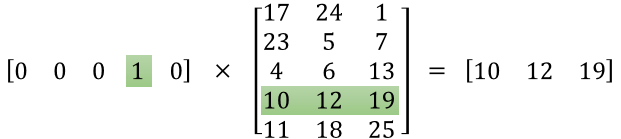
\includegraphics[width=0.8\linewidth]{./img/skip_gram_matrix}
\end{center}

\vspace{0.5cm}

\begin{itemize}
\item a high-level illustration of the architecture:
\end{itemize}

\begin{center}
        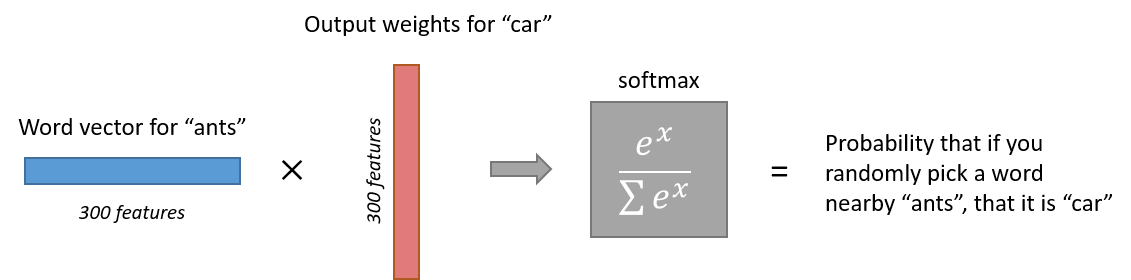
\includegraphics[width=1\linewidth]{./img/skip_gram2}
\end{center}

\footnotesize{Source: \href{https://israelg99.github.io/2017-03-23-Word2Vec-Explained/}{A nice technical tutorial}}
\end{frame}

\begin{frame}{W2V: Problems?}
\begin{center}
          \alert{\textbf{Will similar words have similar vectors?}}
 \end{center}
 
\begin{itemize}
\item  Consider the following sentences: 

 \begin{enumerate}
\item I like watching movies.
\item I enjoy watching movies.
\item I hate watching movie.
\end{enumerate}
\end{itemize}

\begin{itemize}
\item What is the distance between \emph{like}, \emph{enjoy}, and \emph{hate}?
\end{itemize}

\vspace{0.2cm}
\begin{itemize}
\item \visible<2->{How similar are the following sentences?}
\end{itemize}
\visible<2->{
  \begin{enumerate}
\item I like pancakes.
\item Steven enjoys cookies.
\end{enumerate}
}
\end{frame}



\begin{frame}{An Observation on Frequencies: Zipf's Law}
    \begin{columns}
        \column{.5\linewidth}    
        \begin{itemize}
            \item Word models care about word frequency.
            \item But there is a problem\ldots
        \end{itemize}
        %
        \begin{alertblock}{Zipf's Law}
            The frequency of a type is inversely proportional to its rank.
        \end{alertblock}

        \column{.38\linewidth}    
        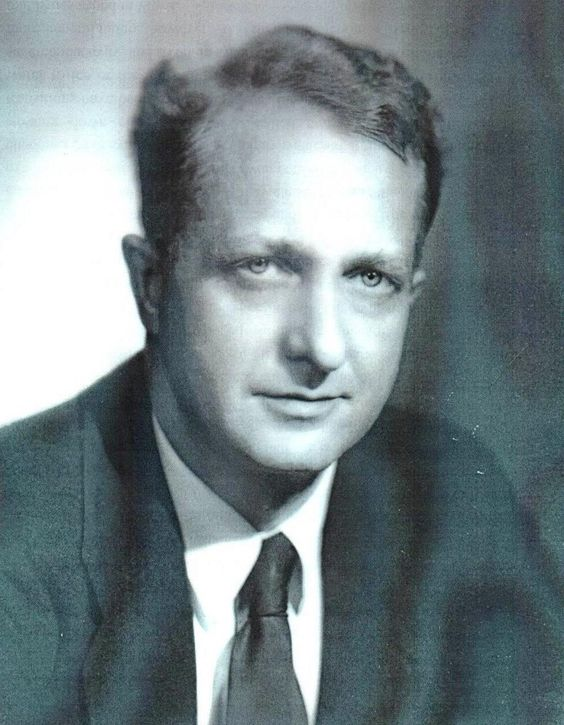
\includegraphics[width=.8\linewidth]{./img/george_zipf}
    \end{columns}

    \pause
    \begin{block}{In Plain English}
        The most frequent word is
            \begin{itemize}
                \item \colored{blue!75}{\textbf{2}} times as common as the \colored{blue!75}{\textbf{2}}nd most frequent word,
                \item \colored{orange}{\textbf{3}} times as common as the \colored{orange}{\textbf{3}}rd most frequent word,
                \item and so on.
            \end{itemize}
    \end{block}
\end{frame}

\begin{frame}{An Example from\ldots the NBA?}
    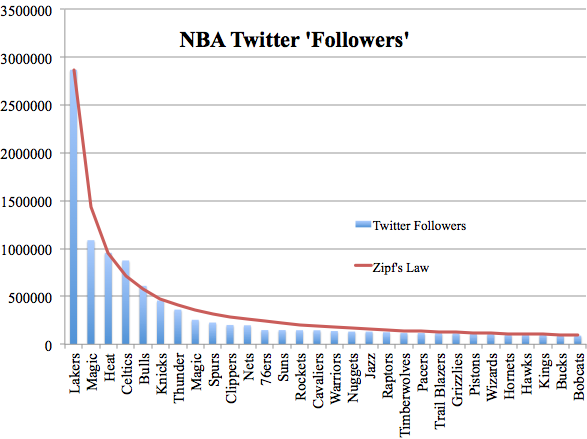
\includegraphics[width=.9\linewidth]{./img/zipfgraph_nba}
\end{frame}


\begin{frame}{Visualizing Zipf Distributions}
    \centering
    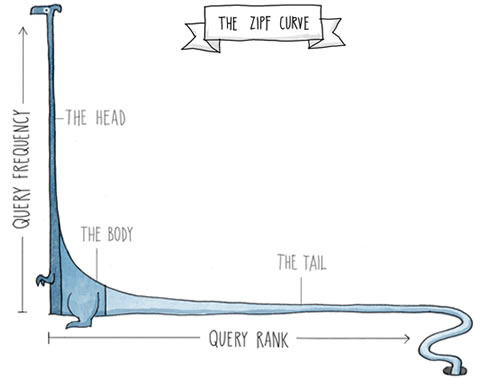
\includegraphics[width=.8\linewidth]{./img/zipfgraph_dinosaur}
\end{frame}

\begin{frame}{Zipf's Law is Everywhere\ldots}
    \begin{itemize}
        \item A distribution is probably Zipfian if
            \begin{itemize}
                \item there is a \highlight{long neck}:\\
                    a few types make up the majority of tokens,
                \item there is a \highlight{long tail}:\\
                    most types only have 1 token (\textbf{hapax legomenon})
            \end{itemize}
        \item Surprisingly, Zipf's Law shows up in tons of places:
            \begin{itemize}
                \item size of large cities in a country
                \item citations for academic papers
                \item frequencies of last names
                \item frequencies of weekdays in text
            \end{itemize}
    \end{itemize}
\end{frame}

\begin{frame}{\ldots Even in Language!}
    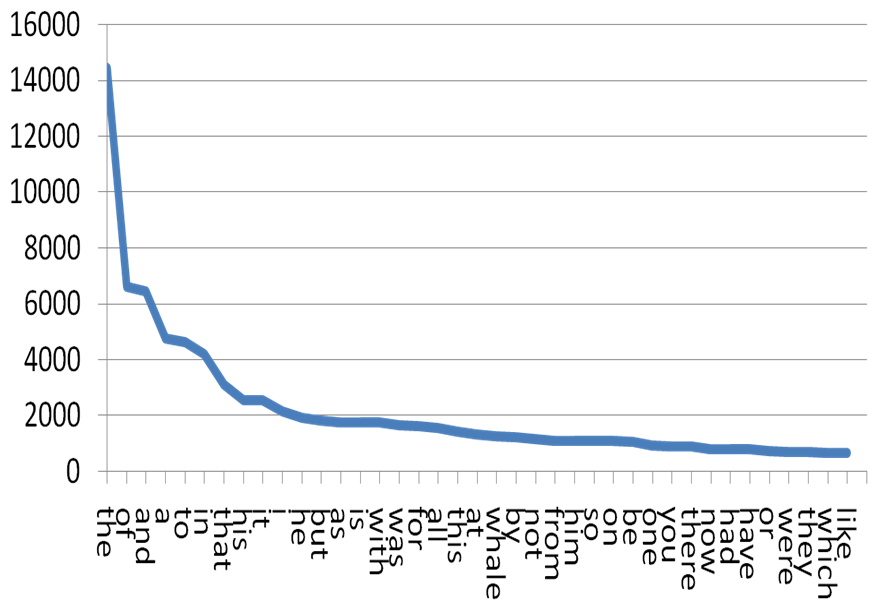
\includegraphics[width=.9\linewidth]{./img/zipfgraph_english}
\end{frame}

\begin{frame}{Stop Words}
    \begin{itemize}
        \item About 150 words make up 50\% of all English texts:\\
            \emph{the}, \emph{of}, \emph{and}, \emph{a}, \ldots
        \item These are called \highlight{stop words}.
        \item Stop words are not very informative for many applications.
        \item So they are usually discarded after the tokenization step.
        \item Failure to do so can greatly reduce the model's performance. 
    \end{itemize}

    \pause
    \begin{block}{Steps of Word Counting Model (Revised)}
        \begin{enumerate}
            \item collect corpus
            \item remove stop words
            \item tokenize strings
            \item count tokens for each type
        \end{enumerate}
    \end{block}
\end{frame}

\begin{frame}{Example: A Text Without (Non)-Stop Words}
    \begin{itemize}
        \item Stop words are much less informative than non-stop words.
        \item Just check the example below.
    \end{itemize}

    \only<1>{\textbf{Stop Words only}}%
    \only<2>{\textbf{Stop Words and Non-Stop Words}}%
    \only<3>{\textbf{Non-Stop Words only}}%

    \bigskip
    \visible<1,2>{The}
    \visible<2,3>{sun}
    \visible<2,3>{shone}
    \visible<1,2>{having}
    \visible<1,2>{no}
    \visible<2,3>{alternative}
    \visible<1,2>{on}
    \visible<1,2>{the}
    \visible<2,3>{nothing}
    \visible<2,3>{new}
\end{frame}

\begin{frame}{An Important Consequence of Zipf's Law}
    \begin{itemize}
        \item Texts mostly consist of stop words.
        \item Hence it can be difficult to get representative counts\\
            for non-stop words.
    \end{itemize}
    %
    \begin{block}{Sparse Data Problem}
        \begin{itemize}
            \item Most of the data is not informative.
            \item You need tons of data to have enough useful data.
        \end{itemize}
    \end{block}
    %
    \visible<2>{
    \begin{example}
        \begin{itemize}
            \item Most models require corpora with at least\\
                a few million sentences.
            \item Really good models (e.g. Google translate) use\\
                billions of data points.
        \end{itemize}
    \end{example}
    }
\end{frame}
\end{document}

